% !TEX root =../main.tex
%%%%%%%%%%%%%%%%%%%%%%%%%%%%%%%%%%%%%%%%%%%%%%%%%%%%%%%%%%%%%%%%%%%%%%
\section{Augmented Attribute-Based Encryption}\label{ABE}
%%%%%%%%%%%%%%%%%%%%%%%%%%%%%%%%%%%%%%%%%%%%%%%%%%%%%%%%%%%%%%%%%%%%%%
\anti{This is the ABE scheme of \cite{STOC:GorVaiWee13} but based on $\sf{ss}$-$\LWE$ with short secrets.}

\paragraph{Circuit Representation.} Let $\calC_\lambda$ be a collection of circuits each having $\ell=\ell(\lambda)$ input wires
and one output wire. Define a collection $\calC = \{\calC_\lambda\}_{\lambda\in\NN}$. For each  $C\in \calC_\lambda$, we index the wires of $C$ in the following way. The input wires are indexed $1$ to $\ell$, the internal wires have indices
$\ell+1,\ell+1,\ldots,|C|-1$ and the output wire has index $|C|$, which also denotes the size of the circuit.
We assume that the circuit is composed of arbitrary two-to-one gates. Each gate $g$ is indexed as a tuple $(u, v,w)$ where $u$ and $v$ are the incoming wire indices, and $w > max\{u, v\}$ is the outgoing
wire index. The gate computes the function $g_w : \bit\times\bit\rightarrow \bit$. The fan-out wires in
the circuit are given a single number. That is, if the outgoing wire of a gate feeds into the input of
multiple gates, then all these wires are indexed the same.


\subsection{The Construction}

The attribute-based encryption scheme $\ABE = (\Setup, \Encrypt, \Keygen, \Decrypt)$ based on $\sf{ss}$-$\LWE$ proceeds as follows.
\BI

\item $\Setup(1^\lambda,1^\ell,d_{max})$: Let $d_{max}$ denote an a-priori fixed bound on the depth of the circuit. For each of the $\ell$ input wires, sample two public/secret key pairs. In particular, generate two matrices for each input wire and a a \emph{random} matrix for the output wire. For the
input wires we use the lattice-trapdoor generation algorithm $\TrapGen(1^n,1^m,q)$ that returns a matrix
$A \in \ZZ_q^{n\times m}$ together with a trapdoor matrix $T\in \ZZ^{m\times m}$. More specifically: 

\BI
\item For $i \in [\ell]$ and $b\in\bit$, set $(A_{i,b}, T_{i,b})\leftarrow \TrapGen(1^n,1^m,q)$.
\item For the output wire, choose a random matrix $A_{\out,1} \in \ZZ_q^{n\times m}$.
\EI
Output:
\begin{multicols}{2}
\begin{equation*}
    \mpk:=\left(  
         \begin{split} A_{1,0}~&~~A_{2,0}~~\ldots~~A_{\ell,0} \\
        A_{1,1}~&~~A_{2,1}~~\ldots~A_{\ell,1}~~ A_{\out,1}    
               \end{split}
    \right)
    \end{equation*}\break    
    \begin{equation*}
    \msk:=\left(  
         \begin{split} T_{1,0}~&~~T_{2,0}~~\ldots~~T_{\ell,0} \\
        T_{1,1}~&~~T_{2,1}~~\ldots~T_{\ell,1}~    
               \end{split}
    \right)
    \end{equation*}
\end{multicols}
\item $\Encrypt(\mpk,\id\in\bit^\ell,\mu\in\bit^{n\times m})$: Choose uniformly random $S  \leftarrow \chi^{n\times n}$ and $E_1,\ldots,E_\ell,E_\out\leftarrow\chi^{n\times m}$. For each wire compute the following: 

\BI
\item For $i \in [\ell]$, set $\psi_{i,\id_i}=S\cdot A_{i,\id_i}+E_i$.
\item For the output wire set $\psi_{\out,1}=S\cdot A_{\out,1}+E_\out + \lceil q/2\rceil \mu ~(\mod q)$.
\EI 
Output: 
$$ \ct_{\id}:=(\id,\psi_{1,\id_1},\ldots,\psi_{\ell,\id_\ell},\psi_{\out,1})$$

\item $\Keygen(\msk,C)$: For every non-input wire $w = \ell+1,\ldots,|C|-1$ of the circuit $C$, and every $b\in\bit$ generate
public/secret key pairs:
$$ (A_{w,b}, T_{w,b})\leftarrow \TrapGen(1^n,1^m,q)$$
Set $A_{|C|,1}:=A_{\out,1}$.\\
Furthermore, for the gate $g = (u, v,w)$ with outgoing wire $w$, compute the four recoding keys  for $b,c\in\bit$: \begin{align*}
    \rk^w_{b,c} &:= \begin{bmatrix}
          R_{b,c} \\
          R'_{b,c} \\
         \end{bmatrix} \in \ZZ^{2m\times m}
  \end{align*}
 such that: 





$$A_{u,b}\cdot R_{b,c}+A_{v,c}\cdot R'_{b,c}=A_{w,g_w(b,c)}$$
Output the secret key which is a collection of $4(|C|-\ell)$ recoding keys
$$\sk_C := \big(\rk^w_{b,c}: w\in[\ell+1,|C|],b,c\in\bit \big)$$


\item $\Decrypt(\sk_C, \ct_\id)$ : Evaluate the circuit $C(\id)$, if $C(\id)= 0$ then output $\bot$. If $C(\id)= 1$ then go over the circuit $C$ in a bottom-up fashion. For $w = \ell+1,\ldots,|C|-1$, let
$g = (u, v,w)$ denote the gate with outgoing wire $w$. Suppose wires $u$ and $v$ carry the values $b^*$
and $c^*$, so that wire $w$ carries the value $d^* := g_w(b^*,c^*)$. Compute the following: 

$$\psi_{w,d^*}=[\psi_{u,b^*}||\psi_{v,c^*}] \cdot \rk^w_{b^*,c^*}$$
Since $C(\id)= 1$, $\psi_{|C|,1}$ is computed. Then for $\psi_{|C|,1}=(\psi_{|C|,1}^1,\ldots,\psi_{|C|,1}^{n\times m})$ and $\psi_{\out,1}=(\psi_{\out,1}^1,\ldots,\psi_{\out,1}^{n\times m})$

output the vector $\mu$ where for all $i = 1,\ldots,n\times m$ 

    
    \begin{align*}\mu_i = \begin{cases} 0 & \text{if } |\psi_{\out,1}^i-\psi_{|C|,1}^i|<q/4 \\
                        1                                & otherwise     %
        \end{cases}\end{align*}
\EI



\paragraph{Correctness} If $C(\id)= 1$, then $\psi_{|C|,1}=S\cdot A_{\out,1} +E_0$ for some small $E_0$. Also $\psi_{\out,1}$ is of the same form, except for the added term $\lceil q/2\rceil \mu$. Hence, correctness follows.

\BT[\cite{STOC:GorVaiWee13}]
For every $\ell$ and polynomial $d_{max} = d_{max}(\sec)$, let $\cC_{\ell,d_{max}}$ denote a family of
polynomial-size circuits of depth at most $d_{max}$ that take $\ell$ bits of input. Assuming the existence
of a $d_{max}$ LWE two-to-one recoding scheme, there exists a selectively secure attribute-based encryption scheme ABE for
$\cC$.
\ET

\BL[\cite{STOC:GorVaiWee13}]
Assuming $\LWE_{n,q,\chi}$ where $q=n^\Theta(d_{max})$, there is an LWE two-to-one recoding scheme that is correct up to $d_{max}$ levels. 
\EL

\begin{corollary}[\cite{STOC:GorVaiWee13}]
For all $\ell$ and polynomial $d_{max} = d_{max}(\sec)$, there exists a selectively secure attribute-
based encryption scheme ABE for any family of polynomial-size circuits with $\ell$ inputs and depth at
most $d_{max}$, assuming the hardness of $\LWE_{n,q,\chi}$ for sufficiently large $n = poly(\sec, d_{max}), q = n^\Theta(d_{max})$ and some $poly(n)$-bounded error distribution $\chi$.
Moreover, assuming $2^{O(\ell)}$-hardness of $\LWE_{n,q,\chi}$ for parameters $n = poly(\sec, d_{max},\ell)$, and q and $\chi$ as above, the attribute-based encryption scheme ABE is fully secure.
\end{corollary}


\paragraph{$\LWE$ Parameters. }\anti{to be written for the $\sf{ss}$-$\LWE$ assumption}

\remove{
\section{Attribute-Based Encryption via Cascading Cancellations}
\anti{Change the name of this ABE later}
\anti{Note that in this ABE scheme the Encryption algorithm is not given the attribute $\id$, therefore all possible encodings are sent out. }
\BI
\item $\Setup(1^\lambda,1^\ell,d_{max})$: For each of the $\ell$ input wires, sample public/secret key pairs. In particular, generate different matrices for each input wire and a a \emph{random} matrix for the output wire. For the
input wires we use the lattice-trapdoor generation algorithm $\TrapGen(1^n,1^m,q)$. More specifically: 

\BI
\item For $i =1$, $j =1,\ldots,\rho$ and $b\in\bit$, set $(B_{1,b}^j, P_{1,b}^j)\leftarrow \TrapGen(1^n,1^m,q)$ and $(A_{1,b}, T_{1,b})\leftarrow \TrapGen(1^n,1^m,q)$.\anti{the parameter $\rho$ and the $B$ matrices are used for the cascading cancellations}\\
Next choose a string $y\in \{-1,1\}^\rho$ by sampling uniformly random bits $y^j \leftarrow \{1,-1\}$ for $j\leq\rho-1$ and setting $y^\rho = 1$. The first part of the public key
consists of matrices $D_{1,b}^j$ for $j\in[\rho]$ defined as follows:
$$D_{1,b}^j=y^j\cdot B_{1,b}^j\in \ZZ_q^{n\times m}$$ 

Next, select random vectors $h^j\in\ZZ_q^n$ for $j<\rho$ and let $h^\rho=\sum_{j<\rho}y^j\cdot h^j$%\anti{the sum is now equal to 1 instead of 0 (0 was used for Brent-Venkata scheme)}
\item For $i =2,\ldots,\ell$, $j =1,\ldots,\rho$ and $b\in\bit$, set  $(B_{i,b}^j, P_{i,b}^j)\leftarrow \TrapGen(1^n,1^m,q)$ and $(A_{i,b}, T_{i,b})\leftarrow \TrapGen(1^n,1^m,q)$.

\item For the output wire, choose a random matrix $A_{\out,1} \in \ZZ_q^{n\times m}$. %for $b\in\bit$.
\EI
Output the following public/secret key pairs where $j\in[\rho]$: 


\begin{multicols}{2}
\begin{equation*}
    \mpk:=\left(  
         \begin{split} A_{1,0}~&~~A_{2,0}~~\ldots~~A_{\ell,0} \\
        A_{1,1}~&~~A_{2,1}~~\ldots~A_{\ell,1}~~ A_{\out,1}    
               \end{split}
    \right)
    \end{equation*}\break    
    \begin{equation*}
    \msk:=\left(  
         \begin{split} T_{1,0}~&~~T_{2,0}~~\ldots~~T_{\ell,0} \\
        T_{1,1}~&~~T_{2,1}~~\ldots~T_{\ell,1}~    
               \end{split}
    \right)
    \end{equation*}
\end{multicols}

\begin{multicols}{2}
\begin{equation*}
    \mpk':=\left(  
         \begin{split} \{ D_{1,0}^j,h^j\}~&~~\{ B_{2,0}^j\}~~\ldots~~\{ B_{\ell,0}^j\} \\
       \{ D_{1,1}^j,h^j\}~&~~\{ B_{2,1}^j\}~~\ldots~\{ B_{\ell,1}^j\}~~ 
               \end{split}
    \right)
    \end{equation*}\break    
    \begin{equation*}
    \msk':=\left(  
         \begin{split}\{  P_{1,0}^j\}~&~~\{ P_{2,0}^j\}~~\ldots~~\{ P_{\ell,0} ^j\}\\
      \{   P_{1,1}^j\}~&~~\{ P_{2,1}^j\}~~\ldots~\{ P_{\ell,1}^j\}~    
               \end{split}
    \right)
    \end{equation*}
\end{multicols}



\item $\Encrypt(\mpk,\mpk',\mu\in\bit^n)$: Choose uniformly random $C_{1,b},\ldots, C_{\ell,b}  \leftarrow \chi^{n\times n}$ for $b\in\bit$ and $E_{2,b}^j,\ldots,E_{\ell,b}^j\leftarrow\chi^{n\times m}$, $E_{1,b}^j\leftarrow\chi^{n}$ for $j\in[\rho]$ and $e_{1,b},\ldots,e_{\ell,b},e_{\out,b}\leftarrow\chi^{m}$. For each wire compute the following: 

\BI
\item For $i =1$ and $\id_1\in\bit$, set $\phi_{1,\id_1}^j=(B_{\ell,\id_\ell}^{-1,j})^\top (C_{1,x_1} \cdot h^j+E_{1,\id_1}^j)$. %where $T=(B^{-1})^\top$.
\item For $i =2,\ldots,\ell$ and $\id_i\in\bit$, set $\Phi_{i,\id_i}^j=B_{i-1,\id_{i-1}}^{-1,j}\cdot (C_{i,\id_i}\cdot B_{i,\id_i}^j+E_{i,\id_i}^j)$.

\anti{\item For $i =1$ and $\id_1\in\bit$, set $f_{1,\id_1}^j=C_{1,x_1} \cdot h^j+E_{1,\id_1}^j \in \ZZ_q^n$ and set $\phi_{1,\id_1}^j\leftarrow SamplePre(B_{1,\id_1}^j, P_{1,\id_1}^j,\sigma,f_{1,\id_1}^j)$ where for $s \leftarrow {\sc{SamplePre}}(A, T_A, \sigma, u)$ it holds that $A \cdot s = u$.
\item For $i =2,\ldots,\ell$ and $\id_i\in\bit$, set $F_{i,\id_i}^j= C_{i,\id_i}\cdot B_{i,\id_i}^j+E_{i,\id_i}^j \in \ZZ_q^{n\times m}$ and set $\Phi_{i,\id_i}^j\leftarrow SamplePre(B_{i,\id_i}^j, P_{i,\id_i}^j,\sigma,F_{i,\id_i}^j)\in \ZZ_q^{m\times m}$.}
\item For each $\id\in(\id_1,\ldots,\id_\ell)$ compute: $$s_{\id}=\sum_{j\in[\rho]}D^j_{1,\id_1}\cdot (\prod_{2\leq i\leq \ell}\Phi_{i,\id_i}^j)\cdot \phi_{1,\id_1}^j \in \ZZ_q^n$$


%\item For $i =1$ and each $\id\in(\id_1,\ldots,\id_\ell)$, set $\psi_{1,\id_1}=S_\id\cdot A_{1,\id_1}+E_{1,\id_1}$.
\item For $i =1,\ldots,\ell$ and each $\id\in(\id_1,\ldots,\id_\ell)$, set $\psi_{i,\id_i}=s_\id \cdot A_{i,\id_i}+e_{i,\id_i}$.
\item For the output wire set $\psi_{\out,\id}=s_\id \cdot A_{\out,\id}+e_{\out,\id} + \lceil q/2\rceil \mu ~(\mod q)$.


\EI 
Output: 
$$ \ct:=(\{\psi_{i,\id_i},\psi_{\out,\id_i}\}_{i\in[\ell],\id_i\in\bit})$$




\item $\Keygen(\msk, \msk', C)$: For every non-input wire $w = \ell+1,\ldots,|C|-1$ of the circuit $C$, and every $b\in\bit$ generate
public/secret key pairs:
$$ (A_{w,b}, T_{w,b})\leftarrow \TrapGen(1^n,1^m,q)$$
Set $A_{|C|,1}:=A_{\out,1}$.\\
Furthermore, for the gate $g = (u, v,w)$ with outgoing wire $w$, compute the four recoding keys  for $b,c\in\bit$: \begin{align*}
    \rk^w_{b,c} &:= \begin{bmatrix}
          R_{b,c} \\
          R'_{b,c} \\
         \end{bmatrix} \in \ZZ^{2m\times m}
  \end{align*}
 such that: 





$$A_{u,b}\cdot R_{b,c}+A_{v,c}\cdot R'_{b,c}=A_{w,g_w(b,c)}$$
Output the secret key which is a collection of $4(|C|-\ell)$ recoding keys
$$\sk_C := \big(\rk^w_{b,c}: w\in[\ell+1,|C|],b,c\in\bit \big)$$


\item $\Decrypt(\sk_C, \ct)$ : Given $\id$, evaluate the circuit $C(\id)$, if $C(\id)= 0$ then output $\bot$. If $C(\id)= 1$ then go over the circuit $C$ in a bottom-up fashion. For $w = \ell+1,\ldots,|C|-1$, let
$g = (u, v,w)$ denote the gate with outgoing wire $w$. Suppose wires $u$ and $v$ carry the values $b^*$
and $c^*$, so that wire $w$ carries the value $d^* := g_w(b^*,c^*)$. Compute the following: 

$$\psi_{w,d^*}=[\psi_{u,b^*}||\psi_{v,c^*}]\cdot \rk^w_{b^*,c^*}$$
Since $C(\id)= 1$, $\psi_{|C|,1}$ is computed. Then for $\psi_{|C|,1}=(\psi_{|C|,1}^1,\ldots,\psi_{|C|,1}^{n\times m})$ and $\psi_{\out,1}=(\psi_{\out,1}^1,\ldots,\psi_{\out,1}^{n\times m})$

output the vector $\mu$ where for all $i = 1,\ldots,n\times m$ 

    
    \begin{align*}\mu_i = \begin{cases} 0 & \text{if } |\psi_{\out,1}^i-\psi_{|C|,1}^i|<q/4 \\
                        1                                & otherwise     %
        \end{cases}\end{align*}

 \anti{in the witness encryption we will check if the encoding has low norm or not to decide the plaintext}

\EI
}

\newpage

\section{Witness Encryption Scheme}
\subsection{Overview}

A witness encryption solution based on the above ABE scheme is fundamentally problematic since the attribute-string is known to the ABE encryptor. However, in a witness encryption scheme the witness is known only to the decryptor. A naive solution will require from the encryptor, who is not given the attribute-string/witness, to publish both input encodings $L_{A_{i,0}}(S)\approx S\cdot A_{i,0}$ and $L_{A_{i,1}}(S)\approx S\cdot A_{i,1}$ for each input wire $i\in[\ell]$. However, if both input encodings on $S$ for the same input wire are published then security of the ABE scheme will completely break down. In order to overcome this difficulty we will generate the input encodings based on a subset product of multiple $S$'s based on each possible witness. That said, the input encodings for the same input wire will correspond to a different subset product of $S$'s. \anti{we need to give more intuition, this paragraph is not very informative}




\paragraph{Encryption.} Let $\cC$ be the verification circuit. For every input wire $i\in[\ell]$, choose $(A_{1,0},A_{1,1},S_{1,0},S_{1,1}\ldots A_{\ell,0},A_{\ell,1},S_{\ell,0},S_{\ell,1}$) and for every internal wire $\ell+1,\ell+2,\ldots,|\cC|$ choose $(A_{\ell+1,0},A_{\ell+1,1}\ldots A_{|\cC|,0},A_{|\cC|,1}$).
Consider an input gate $G$ (say an AND gate) with input wires $i$ and $i+1$ and output wire $k$. 


  {  \centering
    \resizebox{0.3\textwidth}{!}{%

\begin{tikzpicture}[circuit logic US]

  
  
  \node[and gate US, draw,rotate=90,logic gate inputs=nn,text height=1.5cm] at (0,0) (xandy) {};
  \node (G) at (0,0)  {$G$};
  
  \node[align=center] at ($(xandy.input 1) - (0.2,1.2)$) (x) {$$};
   \node[align=center] at ($(xandy.input 2) - (-0.2,1.2)$) (y) {$$};
   
   \draw (x) to ($(xandy.input 1)- (0.2,0)$);
     \draw (y) to ($(xandy.input 2)+ (0.2,0)$);
   
   \path (x) node[above left,align=center] {$S_{i,0},A_{i,0}$\\$S_{i,1},A_{i,1}$};
      \path (y) node[above right,align=center] {$S_{i+1,0},A_{i+1,0}$\\$S_{i+1,1},A_{i+1,1}$};
   
     \node at ($(xandy.output) + (0,1.2)$) (z) {$$};
        \draw (z) to ($(xandy.output)$);
  
    \path (z) node[below right,align=center] {$A_{k,0}$\\$A_{k,1}$};
  
  
  % \draw (xandy.output) -- node[above]{$\bar x + \bar y$} ($(xandy) + (1.5, 0)$);
    
    
    \end{tikzpicture}
   }%
   \par
   }
% \caption{Paths for the first input wire with bit value $b_3$. LWE instances for the case where $d_3=\overline b_3$ are not provided and are highlighted with red color.}


Next, we can associate multiple input encodings based on a subset product of the values $\{S_{i,b_i}\}_{i\in[\ell]}$ to each input wire $i\in[\ell]$ with bit value $b_i\in \bit$. More specifically, we can generate $2^\ell$ input encodings $L_{A_{i,b_i}}^{\bfd}$ for each input wire $i\in[\ell]$ with bit value $b_i \in\bit $ and every other wire value $\bfd=\langle{d_j\rangle}_{j \in[\ell]\setminus\{i\}}$ where $d_j \in\bit $ based on $\big(S_{i,b_i},\{S_{j,d_j}\}_{j \in[\ell]\setminus\{i\}}\big)$ in the following way: 


\begin{equation*}
L_{A_{i,b_i}}^{\bfd}\big(S_{i,b_i},\{S_{j,d_j}\}_{j \in[\ell]\setminus\{i\}}\big)\approx \begin{cases}  \prod_{j<i} S_{j,d_j}\cdot S_{i,0}\cdot \prod_{j>i} S_{j,d_j}\cdot A_{i,0}  & \forall d_j\in \bit, b_i=0\\&\\
                      \prod_{j<i} S_{j,d_j}\cdot S_{i,1}\cdot \prod_{j>i} S_{j,d_j}\cdot A_{i,1}                                   & \forall d_j\in \bit, b_i=1     %
        \end{cases}
         \end{equation*}
         
The main guarantees are as follows. For a possible witness $\id=(\id_1,\ldots,\id_\ell)$ the subset product is the same across all $(L_{A_{1,\id_1}}^\bid,\ldots,L_{A_{\ell,\id_\ell}}^\bid)$ as shown in Figure \ref{Linstances} for the case where $\ell=3$. Morover, the subset products must be different across different witnesses. To this end, encodings for the case where $b_i\neq \id_i$ are not provided. 

         
         
         
         
       
%%%%%%%%%%%%%%%%%%%%%%%%%%%%%%%%%%%%%%%%%%
  \begin{figure}[!tbp]

    \resizebox{1.03\textwidth}{!}{%
    \begin{tikzpicture}[scale=0.8]
         
    
       
  

%    \draw[->,dashed] (c3) to (c4);
 %   \draw[->,dashed,color=red,thick] (d3) to (d4);
   
   
    \node[align=center] (a5) at (-8,9) {$\color{blue} S_{1,\id_1}S_{2,\id_2}S_{3,\id_3}A_{1,\id_1}$\\$S_{1, \id_1}S_{2,\overline \id_2}S_{3,\id_3}A_{1, \id_1}$\\$S_{1,\id_1}S_{2,\id_2}S_{3,\overline \id_3}A_{1,\id_1}$\\$S_{1, \id_1}S_{2,\overline \id_2}S_{3,\overline \id_3}A_{1,\id_1}$};

    \node[align=center] (b5) at (-4.5,9) {$\color{red}S_{1,\overline \id_1}S_{2,\id_2}S_{3,\id_3}A_{1,\overline \id_1}$\\$\color{red}S_{1,\overline \id_1}S_{2,\overline \id_2}S_{3,\id_3}A_{1,\overline \id_1}$\\$\color{red}S_{1,\overline \id_1}S_{2,\id_2}S_{3,\overline \id_3}A_{1,\overline \id_1}$\\$\color{red} S_{1,\overline \id_1}S_{2,\overline \id_2}S_{3,\overline \id_3}A_{1,\overline \id_1}$}; 

    
    \node[align=center] (aa5) at (-0.5,9) {$\color{blue}S_{1,\id_1}S_{2, \id_2}S_{3,\id_3}A_{2,\id_2}$\\$S_{1,\overline \id_1}S_{2, \id_2}S_{3,\id_3}A_{2,\id_2}$\\$S_{1,\id_1}S_{2, \id_2}S_{3,\overline \id_3}A_{2, \id_2}$\\$S_{1,\overline \id_1}S_{2, \id_2}S_{3,\overline \id_3}A_{2, \id_2}$};

    \node[align=center] (bb5) at (3,9) {$\color{red}S_{1,\id_1}S_{2,\overline \id_2}S_{3,\id_3}A_{2,\overline \id_2}$\\$\color{red}S_{1,\overline \id_1}S_{2,\overline \id_2}S_{3,\id_3}A_{2,\overline \id_2}$\\$\color{red}S_{1,\id_1}S_{2,\overline \id_2}S_{3,\overline \id_3}A_{2,\overline \id_2}$\\$\color{red}S_{1,\overline \id_1}S_{2,\overline \id_2}S_{3,\overline \id_3}A_{2,\overline \id_2}$}; 
    %\end{scope}
    
    
    
        \node[align=center] (aaa5) at (7,9) {$\color{blue}S_{1,\id_1}S_{2,\id_2}S_{3, \id_3}A_{3, \id_3}$\\$S_{1,\id_1}S_{2,\overline \id_1}S_{3, \id_3}A_{3, \id_3}$\\$S_{1,\overline \id_1}S_{2,\id_2}S_{3, \id_3}A_{3, \id_3}$\\$S_{1,\overline \id_1}S_{2,\overline \id_2}S_{3, \id_3}A_{3, \id_3}$};

    \node[align=center] (bbb5) at (10.5,9) {$\color{red}S_{1,\id_1}S_{2,\id_2}S_{3,\overline \id_3}A_{3,\overline \id_3}$\\$\color{red}S_{1,\id_1}S_{2,\overline \id_2}S_{3,\overline \id_3}A_{3,\overline \id_3}$\\$\color{red}S_{1,\overline \id_1}S_{2,\id_2}S_{3,\overline \id_3}A_{3,\overline \id_3}$\\$\color{red}S_{1,\overline \id_1}S_{2,\overline \id_2}S_{3,\overline \id_3}A_{3,\overline \id_3}$}; 

  \node (G) at (-6.3,7.5)  {$$};
    \node (A) at (-6.3,10.5)  {$$};
      \draw (G) to (A);

  \node (G) at (1.2,7.5)  {$$};
    \node (A) at (1.2,10.5)  {$$};
  \draw (G) to (A);
    %%%%%%%%%%ADDITIONAL PICTURE%%%%%%%%%%%%%%%%

  \node (G) at (8.7,7.5)  {$$};
    \node (A) at (8.7,10.5)  {$$};
      \draw (G) to (A);   
       
  
  %      \draw[->,dashed] (a3) to (b4);
  %  \draw[->,dashed] (b3) to (a4);
%    \draw[->,dashed] (c3) to (c4);
 %   \draw[->,dashed,color=red,thick] (d3) to (d4);

% \node [below=1cm, align=flush center,text width=8cm] at (a1)
  %      {
  %          $M_1$
 %       };
  \end{tikzpicture}
    }%
        \label{Linstances}

    \caption{ Input encodings $L_{A_{i, \id_i}}^\bid, L_{A_{i,\overline \id_i}}^\bid$ $\forall i\in[\ell]$ for the case where $\ell=3$. For example, if $\id=(\id_1,\ldots,\id_\ell)$ then coloured red encodings are not provided to the decryptor and coloured blue encodings, used to run the ABE scheme, share the same subset product.  }
  \end{figure}    
         
Similarly to the ABE scheme in Section \ref{ABE}, our construction provides a ``translation table" such that given $L_{A_{i,\id_i}}^\bid$ and $L_{A_{i+1,\id_{i+1}}}^\bid$ it outputs $L_{A_{k, \id_i\land \id_{i+1}}}^\bid$ for the output wire of gate $G$ without leaking any information about the product of $S$'s. However, encryption of message $\mu$ is treated in a different way than the ABE scheme. In particular, the ABE scheme assigns matrix $A_{\out,1}$ to the output wire, however in this case if $\mu=1$ matrix $A_{\out,1}$ is assigned to the output wire and if $\mu=0$ matrix $U_{\out,1}$ is assigned to the output wire. The encryptor also publishes the final encodings $L_{A_{\out,1}}^\bfd$ for the output wire computed in the following way: 


\begin{equation*}
L_{A_{\out,1}}^{\bfd}\big(S_{1,b_1},\{S_{j,d_j}\}_{j \in[\ell]\setminus\{1\}}\big)\approx \begin{cases} S_{1,0}\cdot \prod_{j>1} S_{j,d_j}\cdot A_{\out,1}  & \forall d_j\in \bit, b_1=0\\&\\
                      S_{1,1}\cdot \prod_{j>1} S_{j,d_j}\cdot A_{\out,1}                                   & \forall d_j\in \bit, b_1=1     %
        \end{cases}
         \end{equation*}


Unfortunately, the encryptor does not know the witness $\id=(\id_1,\ldots,\id_\ell)$ in advance. That said, he cannot provide only the input encodings $L_{A_{i,b_i}}^\bfd$ for which $b_i=\id_i$ and $d_j=\id_j$ for $j\in[\ell]\setminus\{i\}$. Instead, the encryptor could provide all the encodings for all the possible combinations of $b_i$ and $d_j$. Such a solution would require from the encryptor to send an exponential number (in $\ell$) of encodings. In order to overcome this barrier, the encryptor will send a different set of input encodings based on a different set of ${B}$ matrices used during decryption time to generate the input encodings based on the ${A}$ matrices. To this end, the encryptor chooses $4\cdot \ell$ matrices for every input wire $i\in[\ell]$ denoted by $B_{i,b_i,j,d_j}$ i.e., $\{B_{1,0,j,0},B_{1,0,j,1},B_{1,1,j,0},B_{1,1,j,1}\ldots {B_{\ell,0,j,0},B_{\ell,0,j,1},B_{\ell,1,j,0},B_{\ell,1,j,1}}\}_{j\in[\ell]}$.


  {  \centering
    \resizebox{0.57\textwidth}{!}{%
  
\begin{tikzpicture}[circuit logic US]

    \centering
  
  \node[and gate US, draw,rotate=90,logic gate inputs=nn,text height=1.5cm] at (0,0) (xandy) {};
  \node (G) at (0,0)  {$G$};
  
  \node[align=center] at ($(xandy.input 1) - (0.2,2)$) (x) {$$};
   \node[align=center] at ($(xandy.input 2) - (-0.2,2)$) (y) {$$};
   
   \draw (x) to ($(xandy.input 1)- (0.2,0)$);
     \draw (y) to ($(xandy.input 2)+ (0.2,0)$);
   
   \path (x) node[above left,align=right] {$S_{i,0},A_{i,0}$\\$S_{i,1},A_{i,1}$\\$ \{B_{i,0,j,0},B_{i,0,j,1}$\\~~~~~~~~$B_{i,1,j,0},B_{i,1,j,1}\}_{j\in[\ell]}$};
      \path (y) node[above right,align=left] {$S_{i+1,0},A_{i+1,0}$\\$S_{i+1,1},A_{i+1,1}$\\$ \{B_{i+1,0,j,0},B_{i+1,0,j,1}$\\$~B_{i+1,1,j,0},B_{i+1,1,j,1}\}_{j\in[\ell]}$};
   
     \node at ($(xandy.output) + (0,1.2)$) (z) {$$};
        \draw (z) to ($(xandy.output)$);
  
    \path (z) node[below right,align=center] {$A_{k,0}$\\$A_{k,1}$};
  
  
  % \draw (xandy.output) -- node[above]{$\bar x + \bar y$} ($(xandy) + (1.5, 0)$);
    

    \end{tikzpicture}

   }%
   \par
}
% \caption{Paths for the first input wire with bit value $b_3$. LWE instances for the case where $d_3=\overline b_3$ are not provided and are highlighted with red color.}

In particular, for each input wire $i\in[\ell]$ and $j\in[2,\ldots,\ell]$ the encryptor generates $8\ell^2-\ell$ input encodings $L_{B_{i,b_i,j,d_j}}^{d_{j-1}}$ based on $S_{j-1,d_{j-1}}$ and $4\ell$ input encodings $L_{A_{i,b_i}}^{d_{\ell}}$ based on $S_{\ell,d_{\ell}}$ where $b_i,d_j\in\bit$ for ${i,j\in[\ell]}$ in the following way: 

%$j=\{2,\ldots, \ell\}$

\begin{equation*}
L_{B_{i,b_i,j,d_j}}^{d_{j-1}}\big(S_{j-1,d_{j-1}}\big)\approx  B_{i,b_i,j-1,d_{j-1}}^{-1}S_{j-1,d_{j-1}}B_{i,b_i,j,d_{j}} 
         \end{equation*}

\begin{equation*}
L_{A_{i,b_i}}^{d_{\ell}}\big(S_{\ell,d_{\ell}}\big)\approx B_{i,b_i,\ell,d_{\ell}}^{-1}S_{\ell,d_{\ell}}A_{i,b_i}  \end{equation*}


Similar to the input encodings, the output encodings $L_{A_{\out,1}}^{d_{\ell}}$ must be generated via a sequence of $L_{\hB_{1,b_1,j,d_j}}^{d_{j-1}}$ and $L_{A_{\out,1}}^{d_{\ell}}$ output encodings based on the same $S_{j-1,d_{j-1}}$ and on a different set of matrices $\{\hB_{1,b_1,j,d_j}\}_{j\in[\ell]}$ and $A_{\out,1}$. 

\paragraph{Decryption.} Given a witness $\id=(\id_1,\ldots,\id_\ell)$, matrices $\{B_{i,b_i,1,d_1}\}_{i\in[\ell]}$ and input encodings $\{L_{B_{i,b_i,j,d_j}}^{d_{j-1}}\}_{i\in[\ell],j\in\{2,\ldots,\ell\}}$ for which $b_i=\id_i$ and $\{d_j=\id_j\}_{j\in[\ell]}$ the decryption procedure computes for each input wire $i\in[\ell]$ the following sequences:  
\begin{equation}\label{mult}
\Big\{B_{i,x_i,1,x_1}\cdot L_{B_{i,x_i,2,x_2}}^{x_{1}}\cdot L_{B_{i,x_i,3,x_3}}^{x_{2}}\cdot\ldots\cdot L_{B_{i,x_i,\ell,x_\ell}}^{x_{\ell-1}}\cdot L_{A_{i,x_i}}^{x_{\ell}}\approx L_{A_{i,x_i}}^{\bid}\Big\}_{i\in[\ell]}
   \end{equation}


Given the input encodings $\{L_{A_{i,x_i}}^{\bid}\}$ the encoding of the output wire $L_{A_{|\cC|,1}}^{\bid}$ is generated via the translation tables. If $L_{A_{|\cC|,1}}^{\bid}\approx L_{A_{\out,1}}^{\bid}$ then $\mu=1$ otherwise $\mu=0$. 





%$$\Big\{B_{i,b_i,1,d_1}\cdot L_{B_{i,b_i,2,d_2}}^{d_{1}}\cdot L_{B_{i,b_i,3,d_3}}^{d_{2}}\cdot\ldots\cdot L_{A_{i,b_i}}^{d_{\ell-1}}= L_{A_{i,b_i}}^{\bfd}\Big\}_{i\in[\ell]}$$

% \anti{mention how we encrypt a message $\mu$}

\paragraph{Adds on.}
For a possible witness $\id=(\id_1,\ldots,\id_\ell)$, sequences in equation (\ref{mult}) lead to $\{L^\id_{A_{i,\id_i}}\}_{i\in[\ell]}$ input encodings based on the same subset product. To guarantee that the subset products are different across different witnesses, we enhance our encryption procedure. More specifically, for each input wire $i\in[\ell]$ and $j\in[2,\ldots,\ell]$ the encryptor does not provide the following input encodings where $\{b_i,d_j\}_{i,j\in[\ell]}\in\bit$ for the case where $i=j-1$ and $d_{j-1}\neq b_{i}$:

 \begin{equation}\label{rejB}
\Rej_B:=\Big\{{\color{red}L_{B_{i,b_i,j,d_j}}^{d_{j-1}}}\Big | i = j-1\land d_{j-1} \neq b_i, i\in[\ell], j\in[\ell]\setminus \{1\}\Big\}
         \end{equation}
         
          \begin{equation}\label{rejA}
\Rej_A:=\Big\{{\color{red}L_{A_{i,b_i}}^{d_{\ell}}}\Big | i = j-1\land d_{\ell} \neq b_i, i\in[\ell]\Big\}
         \end{equation}
         
         
         
      \remove{   
         \begin{equation*}
         {\color{red}
L_{B_{i,b_i,j,d_j}}^{d_{j-1}}\big(S_{j-1,d_{j-1}}\big)}\approx \begin{cases} B_{i,0,j-1,d_{j-1}}^{-1}S_{j-1,d_{j-1}}B_{i,0,j,d_{j}} & b_i=0 \land{\color{red} i=j-1 \land d_{j-1}\neq 0} \\&\\
                      B_{i,1,j-1,d_{j-1}}^{-1}S_{j-1,d_{j-1}}B_{i,1,j,d_{j}}                          &b_i=1 \land {\color{red} i=j-1 \land d_{j-1}\neq 1} %
        \end{cases}
         \end{equation*}
         \begin{equation*}
{\color{red}L_{A_{i,b_i}}^{d_{\ell}}\big(S_{\ell,d_{\ell}}\big)}\approx \begin{cases} B_{i,0,\ell,d_{\ell}}^{-1}S_{\ell,d_{\ell}}A_{i,0} & 
 b_i=0 \land{\color{red} d_{\ell}\neq 0}\\&\\
                      B_{i,1,\ell,d_{\ell}}^{-1}S_{\ell,d_{\ell}}A_{i,1}                          & b_i=1 \land{\color{red} d_{\ell}\neq 1}  %
        \end{cases}
         \end{equation*}}
Furthermore, the encryptor does not provide matrices $\{B_{1,b_1,1,d_1}\}_{b_1,d_1\in\bit}$ for the case where $d_1\neq b_1$. Similarly, the matrices $\{\hB_{1,b_1,1,d_1}\}_{b_1,d_1\in\bit}$ and output encodings for the case where $d_1\neq b_1$ are not provided:
  
  
   \begin{equation}\label{rejhB}
\Rej_\hB:=\Big\{{\color{red}L_{\hB_{1,b_1,j,d_j}}^{d_{j-1}}}\Big | j-1=1\land d_{j-1} \neq b_1, j\in[\ell]\setminus \{1\}\Big\}
         \end{equation}
         
          \begin{equation}\label{rejAout}
\Rej_{A_{\out}}:=\Big\{{\color{red}L_{A_{\out,1}}^{d_{\ell}}}\Big | d_{\ell} \neq b_1\Big\}
         \end{equation}
      
      In order to have the security proof go through, we introduce additional dimension to the matrices $\{S_{j,b_j}\}_{j\in[\ell]}$ which will be null in the real execution but will gradually change values via a sequence of hybrids in the security proof. Since the values of $\{S_{j,b_j}\}_{j\in[\ell]}$ are null on the extra dimensions then encodings based on $\{S_{j,b_j}\}_{j\in[\ell]}$ will be distinghuisable. For this reason we introduce a set of $\{V_j\}_{j\in[\ell]}$ matrices to mask matrices $\{S_{j,b_j}\}_{j\in[\ell]}$. In particular, each encoding is computed as follows: %\anti{check how many extra dimensions we need}
      
      
      \begin{equation*}
L_{B_{i,b_i,j,d_j}}^{d_{j-1}}\big(S_{j-1,d_{j-1}}\big)\approx  B_{i,b_i,j-1,d_{j-1}}^{-1}V_{j-1}^{-1}S_{j-1,d_{j-1}}V_{j}B_{i,b_i,j,d_{j}} 
         \end{equation*}   
  
  \begin{equation*}
L_{A_{i,b_i}}^{d_{\ell}}\big(S_{\ell,d_{\ell}}\big)\approx B_{i,b_i,\ell,d_{\ell}}^{-1}V_{\ell}^{-1}S_{\ell,d_{\ell}}A_{i,b_i}  \end{equation*}
  
Output encodings $L_{\hB_{1,b_1,j,d_j}}^{d_{j-1}}$, $L_{A_{\out,1}}^{d_{\ell}}$ are generated in a similar fashion based on lower unitriangular matrices $V_{0},\ldots, V_\ell  \leftarrow \chi^{n\times n}$. In addition, matrices $\{B_{i,b_i,j,d_j}\}_{j\in[\ell]}$ and $\{\hB_{i,b_i,j,d_j}\}_{j\in[\ell]}$ are multiplied on the left by matrix $V_0$.   
\paragraph{Example for $\ell=3$.}
In the following we provide a detailed example for $\ell=3$. We first present the assignment of matrices for gates $G,G'$ and in Figures \ref{ell1} and \ref{ell3} we show the corresponding encodings. Notice that the subset products across all $\{L_{A_{i,\id_i}}^\bid\}_{i\in[3]}$ for a possible witness $\bid=(\id_1,\ldots,\id_\ell)$ are the same. On the other hand, the subset products 
between $L_{A_{i,\id_i}}^\bid$ and $L_{A_{i,\bar \id_i}}^\bid$ for all $i\in[3]$ are different. 

  {  \centering
    \resizebox{1.04\textwidth}{!}{%

\begin{tikzpicture}[circuit logic US]

  
  
  \node[and gate US, draw,rotate=90,logic gate inputs=nn,text height=1.5cm] at (-4,0) (xandy) {};
  
    
  \node[and gate US, draw,rotate=90,logic gate inputs=nn,text height=1.5cm] at (4,0) (xxandy) {};
  \node (G) at (-4,0)  {$G$};
    \node (G2) at (4,0)  {$G'$};
  
  \node[align=center] at ($(xandy.input 1) - (0,2.5)$) (x) {$$};
   \node[align=center] at ($(xandy.input 2) - (0,2.5)$) (y) {$$};
   
   \draw (x) to ($(xandy.input 1)$);
     \draw (y) to ($(xandy.input 2)$);
   
   \path (x) node[above left,align=right] {$S_{1,b_1},A_{1,b_1}$\\$S_{1,\overline b_1},A_{1,\overline b_1}$\\$ B_{1,b_1,1,0},B_{1,b_1,1,1},B_{1,\overline b_1,1,0},B_{1,\overline b_1,1,1}$\\$ B_{1,b_1,2,0},B_{1,b_1,2,1},B_{1,\overline b_1,2,0},B_{1,\overline b_1,2,1}$\\$ B_{1,b_1,3,0},B_{1,b_1,3,1},B_{1,\overline b_1,3,0},B_{1,\overline b_1,3,1}$};
      \path (y) node[above right,align=left] {$S_{2,b_2},A_{2,b_2}$\\$S_{2,\overline b_2},A_{2,\overline b_2}$\\$B_{2,b_2,1,0},B_{2,b_2,1,1},B_{2,\overline b_2,1,0},B_{2,\overline b_2,1,1}$\\$B_{2,b_2,2,0},B_{2,b_2,2,1},B_{2,\overline b_2,2,0},B_{2,\overline b_2,2,1}$\\$B_{2,b_2,3,0},B_{2,b_2,3,1},B_{2,\overline b_2,3,0},B_{2,\overline b_2,3,1}$};
   
      
  \node[align=center] at ($(xxandy.input 2) - (0.3,2.5)$) (xx) {$$};
%   \node[align=center] at ($(xxandy.input 2) - (0,2)$) (yy) {$$};
   
   \draw (xx) to ($(xxandy.input 2)- (0.3,0)$);
 %    \draw (yy) to ($(xxandy.input 2)$);
   
   \path (xx) node[above right,align=left] {$S_{3,b_3},A_{3,b_3}$\\$S_{3,\overline b_3,},A_{3,\overline b_3}$\\$B_{3,b_3,1,0},B_{3,b_3,1,1},B_{3,\overline b_3,1,0},B_{3,\overline b_3,1,1}$\\$B_{3,b_3,2,0},B_{3,b_3,2,1},B_{3,\overline b_3,2,0},B_{3,\overline b_3,2,1}$\\$B_{3,b_3,3,0},B_{3,b_3,3,1},B_{3,\overline b_3,3,0},B_{3,\overline b_3,3,1}$};

         \node at ($(xandy.output) + (0,0.5)$) (z) {$$};
        \draw (z) to ($(xandy.output)$);
      \node at ($(xxandy.output) + (0,0.5)$) (zz) {$$};
        \draw (zz) to ($(xxandy.output)$);

    
    \end{tikzpicture}
   }%
   \par
   }
% \caption{Paths for the first input wire with bit value $b_3$. LWE instances for the case where $d_3=\overline b_3$ are not provided and are highlighted with red color.}

%%%%%%%%%%%%%%%%%%%pictures%%%%%%%%%%%%%%%%%%%%%%%%%


%%%%%%%%%%%%%%%%%%%%%%%%%%%%%%%%%%%%%%%%%%
  \begin{figure}[!tbp]
\centering
    \resizebox{0.88\textwidth}{!}{%
    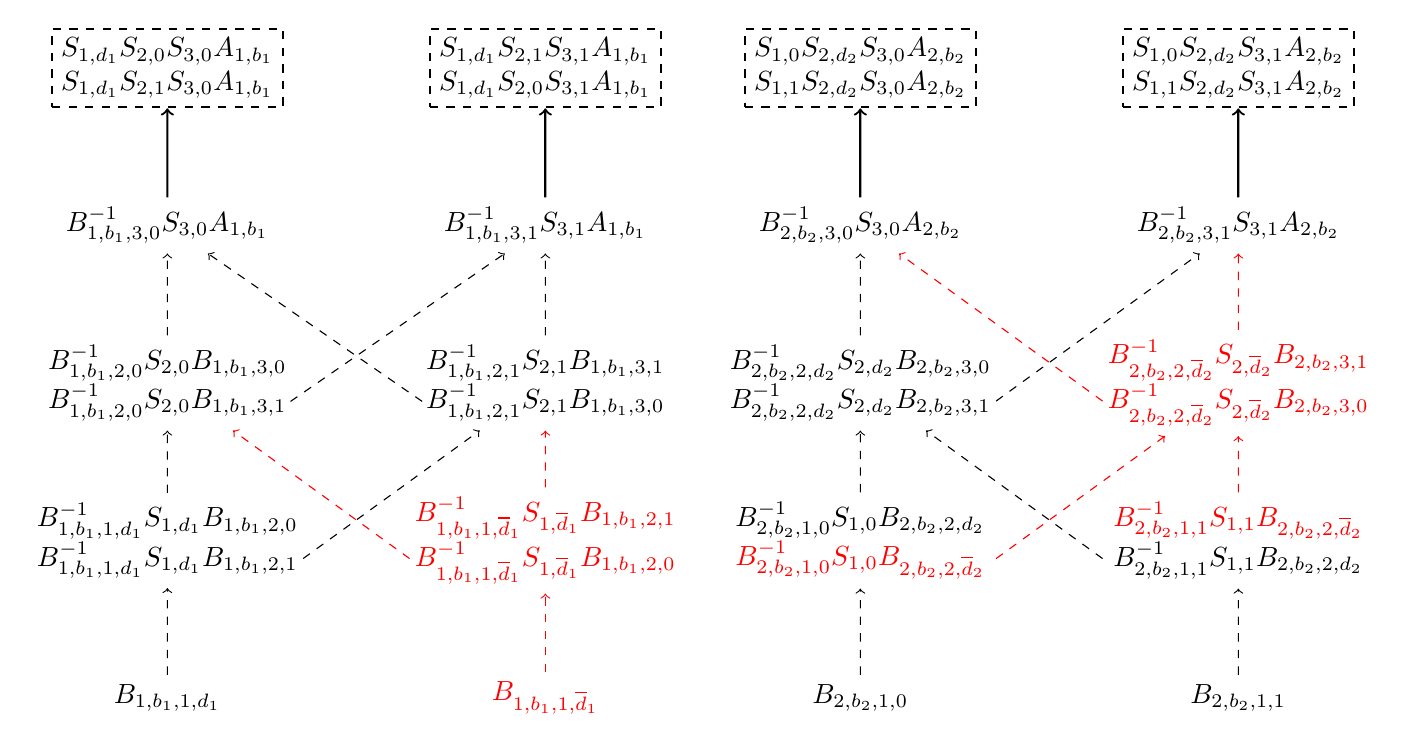
\begin{tikzpicture}[scale=0.8]
      \node (a1) at (-7,0) {$B_{1,b_1,1,d_1}$};
          \node[color=red] (b1) at (-1,0) {$B_{1,b_1,1,\overline d_1}$};
    \node[align=center]  (a2) at (-7,2.5) {$B_{1,b_1,1,d_1}^{-1}S_{1,d_1}B_{1,b_1,2,0}$\\$B_{1,b_1,1,d_1}^{-1}S_{1,d_1}B_{1,b_1,2,1}$};
        \node[align=center,color=red]  (b2) at (-1,2.5) {$B_{1,b_1,1,\overline d_1}^{-1}S_{1,\overline d_1}B_{1,b_1,2,1}$\\$B_{1,b_1,1,\overline d_1}^{-1}S_{1,\overline d_1}B_{1,b_1,2,0}$};


     \node (a'2) at (-5,2.1) {$$};
          \node (b'2) at (-3,2.1) {$$};
    
    
    %\path (0,1) node {\dots};
    %\path (a2) to node[midway] {\dots} (b2);
    
    \draw[->,dashed] (a1) to (a2);
        \draw[->,dashed,color=red] (b1) to (b2);
        

    
    \node (a3)[align=center] at (-7,5) {$B_{1,b_1,2,0}^{-1}S_{2,0}B_{1,b_1,3,0}$\\$B_{1,b_1,2,0}^{-1}S_{2,0}B_{1,b_1,3,1}$};

    \node (b3)[align=center]  at (-1,5) {$B_{1,b_1,2,1}^{-1}S_{2,1}B_{1,b_1,3,1}$\\$B_{1,b_1,2,1}^{-1}S_{2,1}B_{1,b_1,3,0}$}; 

    
         \node (a'3) at (-5.2,4.6) {$$};
          \node (b'3) at (-2.8,4.6) {$$};
    
    
    \draw[->,dashed] (a2) to (a3);
    \draw[->,dashed] (a'2) to (b3);
        
    \draw[->,dashed,color=red] (b2) to (b3);
    \draw[->,dashed,color=red] (b'2) to (a3);

   
    
    %\begin{scope}[yshift=3cm]
    

  %   \node (a4) at (-2.25,4.5) {$B_{1,b_1,3,0}^{-1}S_{3,0}A_{1,b_1}$};
%    \node (b4) at (-0.75,4.5) {$B_{1,b_1,3,1}^{-1}S_{3,1}A_{1,b_1}$};
 %   \node (c4) at (0.75,4.5) {$B_{1,b_1,3,0}^{-1}S_{3,0}A_{1,b_1}$}; 
  %  \node (d4) at (2.25,4.5) {$B_{1,b_1,3,1}^{-1}S_{3,1}A_{1,b_1}$}; 
    

    
    
    \node(a4) at (-7,7.5) {$B_{1,b_1,3,0}^{-1}S_{3,0}A_{1,b_1}$};
  \node (b4) at (-1,7.5) {$B_{1,b_1,3,1}^{-1}S_{3,1}A_{1,b_1}$};
   
       
    \draw[->,dashed] (a3) to (a4);
    \draw[->,dashed] (b3) to (b4);
    
           
    \draw[->,dashed] (a'3) to (b4);
    \draw[->,dashed] (b'3) to (a4);

%    \draw[->,dashed] (c3) to (c4);
 %   \draw[->,dashed,color=red,thick] (d3) to (d4);
   
   
    \node[draw,rectangle,thick,dashed,align=center] (a5) at (-7,10) {$S_{1,d_1}S_{2,0}S_{3,0}A_{1,b_1}$\\$S_{1,d_1}S_{2,1}S_{3,0}A_{1,b_1}$};

    \node[draw,rectangle,thick,dashed,align=center] (b5) at (-1,10) {$S_{1,d_1}S_{2,1}S_{3,1}A_{1,b_1}$\\$S_{1,d_1}S_{2,0}S_{3,1}A_{1,b_1}$}; 

    
    
    %\end{scope}

    
    \draw[->,thick] (a4) to (a5);
    \draw[->,thick] (b4) to (b5);

    %%%%%%%%%%ADDITIONAL PICTURE%%%%%%%%%%%%%%%%
    
          \node (aa1) at (4,0) {$B_{2,b_2,1,0}$ };
            \node (bb1) at (10,0) {$B_{2,b_2,1,1}$ };
    \node[align=center] (aa2) at (4,2.5) {$B_{2,b_2,1,0}^{-1}S_{1,0}B_{2,b_2,2,d_2}$\\$\color{red}B_{2,b_2,1,0}^{-1}S_{1,0}B_{2,b_2,2,\overline d_2}$};
    \node[align=center] (bb2) at (10,2.5) {$\color{red}B_{2,b_2,1,1}^{-1}S_{1,1}B_{2,b_2,2, \overline d_2}$\\$B_{2,b_2,1,1}^{-1}S_{1,1}B_{2,b_2,2, d_2}$};
    

     \node (aa'2) at (6,2.1) {$$};
          \node (bb'2) at (8,2.1) {$$};
    

    %\path (0,1) node {\dots};
    %\path (a2) to node[midway] {\dots} (b2);
    
    \draw[->,dashed] (aa1) to (aa2);
     \draw[->,dashed] (bb1) to (bb2);
    
    \node[align=center] (aa3) at (4,5) {$B_{2,b_2,2,d_2}^{-1}S_{2,d_2}B_{2,b_2,3,0}$\\$B_{2,b_2,2,d_2}^{-1}S_{2,d_2}B_{2,b_2,3,1}$};
    \node[align=center,color=red] (bb3) at (10,5) {$B_{2,b_2,2,\overline d_2}^{-1}S_{2,\overline d_2}B_{2,b_2,3,1}$\\$B_{2,b_2,2,\overline d_2}^{-1}S_{2,\overline d_2}B_{2,b_2,3,0}$};
                 \node (aa'3) at (6,4.6) {$$};
          \node (bb'3) at (8,4.6) {$$};
 
 %   \node (c3) at (1.65,5) {$B_{2,b_2,2,b_2}^{-1}S_{2,b_2}B_{2,b_2,3,0}$}; 
   % \node (d3) at (5,5) {$B_{2,b_2,2,b_2}^{-1}S_{2,b_2}B_{2,b_2,3,1}$}; 
    
    \draw[->,dashed] (aa2) to (aa3);
    \draw[->,dashed,color=red] (aa'2) to (bb3);
    \draw[->,dashed] (bb'2) to (aa3);
    \draw[->,dashed,color=red] (bb2) to (bb3);
    

    
    %\begin{scope}[yshift=3cm]
    

  %   \node (a4) at (-2.25,4.5) {$B_{1,b_1,3,0}^{-1}S_{3,0}A_{1,b_1}$};
%    \node (b4) at (-0.75,4.5) {$B_{1,b_1,3,1}^{-1}S_{3,1}A_{1,b_1}$};
 %   \node (c4) at (0.75,4.5) {$B_{1,b_1,3,0}^{-1}S_{3,0}A_{1,b_1}$}; 
  %  \node (d4) at (2.25,4.5) {$B_{1,b_1,3,1}^{-1}S_{3,1}A_{1,b_1}$}; 
    

    
    
    \node(aa4) at (4,7.5) {$B_{2,b_2,3,0}^{-1}S_{3,0}A_{2,b_2}$};
  \node (bb4) at (10,7.5) {$B_{2,b_2,3,1}^{-1}S_{3,1}A_{2,b_2}$};
   
       
    \draw[->,dashed] (aa3) to (aa4);
    \draw[->,dashed,color=red] (bb3) to (bb4);
        \draw[->,dashed] (aa'3) to (bb4);
    \draw[->,dashed,color=red] (bb'3) to (aa4);
  %      \draw[->,dashed] (a3) to (b4);
  %  \draw[->,dashed] (b3) to (a4);
%    \draw[->,dashed] (c3) to (c4);
 %   \draw[->,dashed,color=red,thick] (d3) to (d4);
   
   
    \node[draw,rectangle,thick,dashed,align=center] (aa5) at (4,10) {$S_{1,0}S_{2,d_2}S_{3,0}A_{2,b_2}$\\$S_{1,1}S_{2,d_2}S_{3,0}A_{2,b_2}$};

    \node[draw,rectangle,thick,dashed,align=center] (bb5) at (10,10) {$S_{1,0}S_{2,d_2}S_{3,1}A_{2,b_2}$\\$S_{1,1}S_{2,d_2}S_{3,1}A_{2,b_2}$}; 

    
    
    %\end{scope}

    
    \draw[->,thick] (aa4) to (aa5);
    \draw[->,thick] (bb4) to (bb5);
    
% \node [below=1cm, align=flush center,text width=8cm] at (a1)
  %      {
  %          $M_1$
 %       };
  \end{tikzpicture}
    }%
        \label{ell1}

    \caption{\footnotesize Input encodings $\{L_{B_{1,b_1,j,d_j}}^{d_{j-1}}\}_{j\in[\ell]}$ ($\{L_{B_{2,b_2,j,d_j}}^{d_{j-1}}\}_{j\in[\ell]}$ ) for the first (second) input wire with bit value $b_1$ ($b_2$) are described on the left (right). Encodings based on $\overline d_1$ ($\overline d_2$) are not provided and are highlighted with red color. The corresponding $L_{A_{1,b_1}}^\bfd, L_{A_{2,b_2}}^\bfd$ encodings are described inside the dashed squares. }
  \end{figure}
  
  
  
%%%%%%%%%%%%%%%%%%%%%%%%%%%%%%%%%%%%%%%%%%
  \begin{figure}[!tbp]
\centering
    \resizebox{0.84\textwidth}{!}{%
    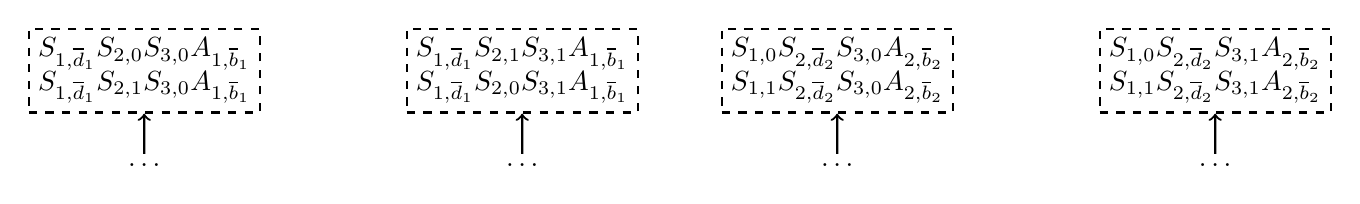
\begin{tikzpicture}[scale=0.8]
         
    
    \node(a4) at (-7,7.5) {$\ldots$};
  \node (b4) at (-1,7.5) {$\ldots$};
   
       
  

%    \draw[->,dashed] (c3) to (c4);
 %   \draw[->,dashed,color=red,thick] (d3) to (d4);
   
   
    \node[draw,rectangle,thick,dashed,align=center] (a5) at (-7,9) {$S_{1,\overline d_1}S_{2,0}S_{3,0}A_{1,\overline b_1}$\\$S_{1,\overline d_1}S_{2,1}S_{3,0}A_{1,\overline b_1}$};

    \node[draw,rectangle,thick,dashed,align=center] (b5) at (-1,9) {$S_{1,\overline d_1}S_{2,1}S_{3,1}A_{1,\overline b_1}$\\$S_{1,\overline d_1}S_{2,0}S_{3,1}A_{1,\overline b_1}$}; 

    
    
    %\end{scope}

    
    \draw[->,thick] (a4) to (a5);
    \draw[->,thick] (b4) to (b5);

    %%%%%%%%%%ADDITIONAL PICTURE%%%%%%%%%%%%%%%%
    
             
    \node(aa4) at (4,7.5) {$\ldots$};
  \node (bb4) at (10,7.5) {$\ldots$};
   
       
  
  %      \draw[->,dashed] (a3) to (b4);
  %  \draw[->,dashed] (b3) to (a4);
%    \draw[->,dashed] (c3) to (c4);
 %   \draw[->,dashed,color=red,thick] (d3) to (d4);
   
   
    \node[draw,rectangle,thick,dashed,align=center] (aa5) at (4,9) {$S_{1,0}S_{2,\overline d_2}S_{3,0}A_{2,\overline b_2}$\\$S_{1,1}S_{2,\overline d_2}S_{3,0}A_{2,\overline b_2}$};

    \node[draw,rectangle,thick,dashed,align=center] (bb5) at (10,9) {$S_{1,0}S_{2,\overline d_2}S_{3,1}A_{2,\overline b_2}$\\$S_{1,1}S_{2,\overline d_2}S_{3,1}A_{2,\overline b_2}$}; 

    
    
    %\end{scope}

    
    \draw[->,thick] (aa4) to (aa5);
    \draw[->,thick] (bb4) to (bb5);
    
% \node [below=1cm, align=flush center,text width=8cm] at (a1)
  %      {
  %          $M_1$
 %       };
  \end{tikzpicture}
    }%
        \label{ell1}

    \caption{ Input encodings $L_{A_{1,\overline b_1}}^\bfd, L_{A_{2,\overline b_2}}^\bfd$ for first and second input wires with bit value $\overline b_1$ and $\overline b_2$, respectively. }
  \end{figure}


%%%%%%%%%%%%%%%%%%%%%%%%%%%%%%%%%%%%%%%%%
  \begin{figure}[!tbp]
    \centering
    \resizebox{0.87\textwidth}{!}{%
    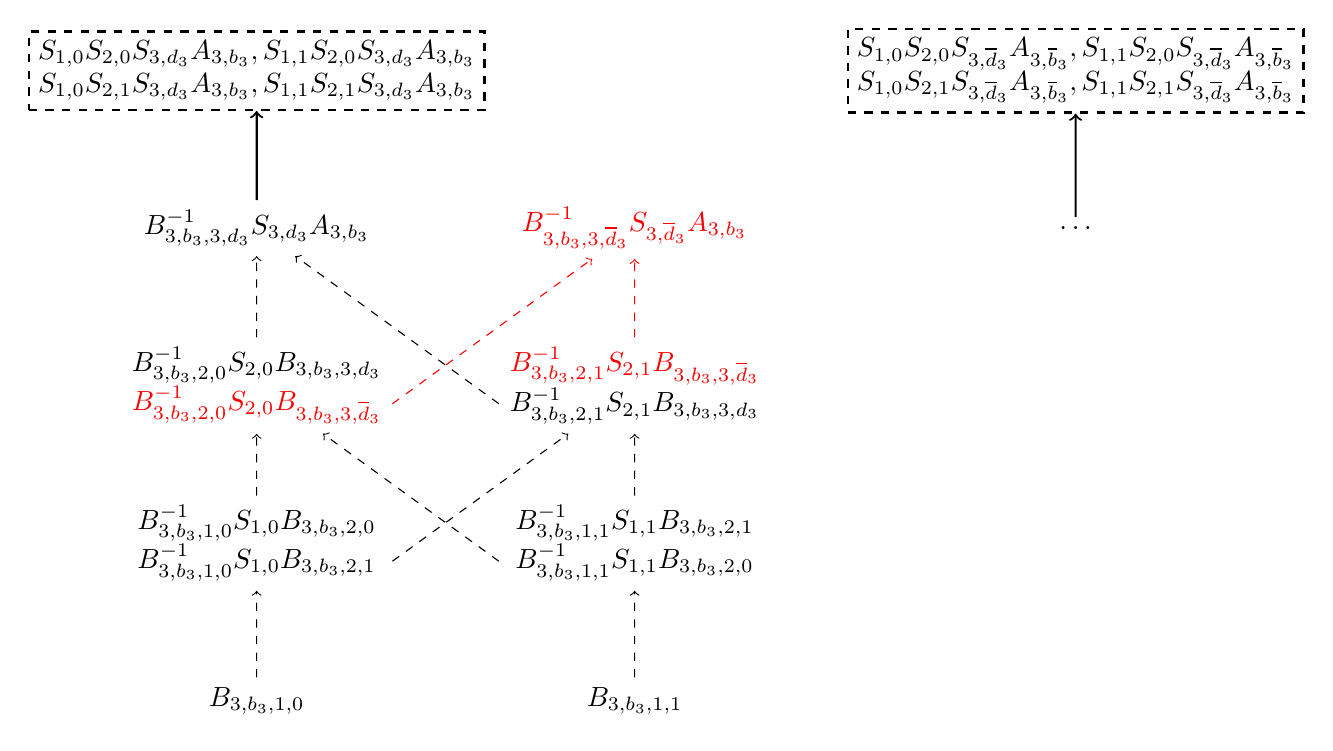
\begin{tikzpicture}[scale=0.8]
      \node (a1) at (-7,0) {$B_{3,b_3,1,0}$ };
            \node (b1) at (-1,0) {$B_{3,b_3,1,1}$ };
    \node[align=center] (a2) at (-7,2.5) {$B_{3,b_3,1,0}^{-1}S_{1,0}B_{3,b_3,2,0}$\\$B_{3,b_3,1,0}^{-1}S_{1,0}B_{3,b_3,2, 1}$};

        \node[align=center] (b2) at (-1,2.5) {$B_{3,b_3,1,1}^{-1}S_{1,1}B_{3,b_3,2, 1}$\\$B_{3,b_3,1,1}^{-1}S_{1,1}B_{3,b_3,2,0}$};
      \node (a'2) at (-5,2.1) {$$};
          \node (b'2) at (-3,2.1) {$$};
    
    %\path (0,1) node {\dots};
    %\path (a2) to node[midway] {\dots} (b2);
    
    \draw[->,dashed] (a1) to (a2);

         \draw[->,dashed] (b1) to (b2);

    
    \node[align=center] (a3) at (-7,5) {$B_{3,b_3,2,0}^{-1}S_{2,0}B_{3,b_3,3,d_3}$\\$\color{red}B_{3,b_3,2,0}^{-1}S_{2,0}B_{3,b_3,3,\overline d_3}$};
    \node[align=center] (b3) at (-1,5) {$\color{red}B_{3,b_3,2,1}^{-1}S_{2,1}B_{3,b_3,3,\overline d_3}$\\$B_{3,b_3,2,1}^{-1}S_{2,1}B_{3,b_3,3,d_3}$};
  
        \node (a'3) at (-5,4.6) {$$};
          \node (b'3) at (-3,4.6) {$$};
    
    \draw[->,dashed] (a2) to (a3);
    \draw[->,dashed] (b2) to (b3);
    \draw[->,dashed] (a'2) to (b3);
    \draw[->,dashed] (b'2) to (a3);
    

    
    %\begin{scope}[yshift=3cm]
    

  %   \node (a4) at (-2.25,4.5) {$B_{1,b_1,3,0}^{-1}S_{3,0}A_{1,b_1}$};
%    \node (b4) at (-0.75,4.5) {$B_{1,b_1,3,1}^{-1}S_{3,1}A_{1,b_1}$};
 %   \node (c4) at (0.75,4.5) {$B_{1,b_1,3,0}^{-1}S_{3,0}A_{1,b_1}$}; 
  %  \node (d4) at (2.25,4.5) {$B_{1,b_1,3,1}^{-1}S_{3,1}A_{1,b_1}$}; 
    

    
    
    \node(a4) at (-7,7.5) {$B_{3,b_3,3,d_3}^{-1}S_{3,d_3}A_{3,b_3}$};
        \node(b4) at (-1,7.5) {$\color{red}B_{3,b_3,3,\overline d_3}^{-1}S_{3,\overline d_3}A_{3,b_3}$};
%  \node (b4) at (3,7.5) {$B_{2,b_2,3,1}^{-1}S_{3,1}A_{2,b_2}$};
   
       
    \draw[->,dashed] (a3) to (a4);
    \draw[->,dashed,color=red] (b3) to (b4);
     \draw[->,dashed,color=red] (a'3) to (b4);
    \draw[->,dashed] (b'3) to (a4);

%    \draw[->,dashed] (c3) to (c4);
 %   \draw[->,dashed,color=red,thick] (d3) to (d4);
   
   
    \node[draw,rectangle,thick,dashed,align=center] (a5) at (-7,10) {$S_{1,0}S_{2,0}S_{3,d_3}A_{3,b_3},S_{1,1}S_{2,0}S_{3,d_3}A_{3,b_3}$\\$S_{1,0}S_{2,1}S_{3,d_3}A_{3,b_3},S_{1,1}S_{2,1}S_{3,d_3}A_{3,b_3}$};

%    \node[draw,rectangle,thick,dashed,align=center] (b5) at (3,10) {$S_{1,0}S_{2,1}S_{3,b_3}A_{3,b_3}$\\$S_{1,1}S_{2,1}S_{3,b_3}A_{3,b_3}$}; 

    
    
    %\end{scope}

    
    \draw[->,thick] (a4) to (a5);
  

    %%%%%%%%%%
     \node(aa4) at (6,7.5) {$\ldots$};
   %     \node(bb4) at (10,7.5) {$\color{red}B_{3,b_3,3,\overline b_3}^{-1}S_{3,\overline b_3}A_{3,b_3}$};
%  \node (b4) at (3,7.5) {$B_{2,b_2,3,1}^{-1}S_{3,1}A_{2,b_2}$};
   


%    \draw[->,dashed] (c3) to (c4);
 %   \draw[->,dashed,color=red,thick] (d3) to (d4);
   
   
    \node[draw,rectangle,thick,dashed,align=center] (aa5) at (6,10) {$S_{1,0}S_{2,0}S_{3,\overline d_3}A_{3,\overline b_3},S_{1,1}S_{2,0}S_{3,\overline d_3}A_{3,\overline b_3}$\\$S_{1,0}S_{2,1}S_{3,\overline d_3}A_{3,\overline b_3},S_{1,1}S_{2,1}S_{3,\overline d_3}A_{3,\overline b_3}$};

%    \node[draw,rectangle,thick,dashed,align=center] (b5) at (3,10) {$S_{1,0}S_{2,1}S_{3,b_3}A_{3,b_3}$\\$S_{1,1}S_{2,1}S_{3,b_3}A_{3,b_3}$}; 

    
    
    %\end{scope}

    
    \draw[->,thick] (aa4) to (aa5);
    
    
    
    

  \end{tikzpicture}
    }%
    \label{ell3}
    \caption{\footnotesize Input encodings $\{L^{d_{j-1}}_{B_{3,b_3,j,d_j}}\}_{j\in[\ell]}$ for the third input wire with bit value $b_3$. Instances that include $\overline d_3$ are not provided and are highlighted with red color. Instances $L_{A_{3,b_3}}^\bfd, L_{A_{3,\overline b_3}}^\bfd$ are described inside the dashed squares.}
  \end{figure}

%%%%%%%%%%%%%%%%%%%pictures%%%%%%%%%%%%%%%%%%%%%%%%%

\newpage


\subsection{Witness Encryption Scheme}

\BI
\item $\Encrypt(1^\lambda,1^\ell,d_{max},\mu\in\bit)$: Let $d_{max}$ denote an a-priori fixed bound on the depth of the verification circuit. \\
{\bf Handling input wires:}
For each of the $\ell$ input wires, sample a sequence of matrices. In particular, generate $4\ell+2$ matrices for each input wire and two \emph{random} matrices for the output wire. For the
input wires we use the lattice-trapdoor generation algorithm $\TrapGen(1^n,1^m,q)$ that returns a matrix
$A \in \ZZ_q^{n\times m}$ together with a trapdoor matrix $T_A\in \ZZ^{m\times m}$. More specifically: 

\BI
\item For $i \in [\ell]$ and $b_i\in\bit$, set $(A_{i,b_i}, T_{A_{i,b_i}})\leftarrow \TrapGen(1^n,1^m,q)$.
\item For $i,j \in [\ell]$ and $b_i,d_j\in\bit$, set $(B_{i,b_i,j,d_j}, T_{B_{i,b_i,j,d_j}})\leftarrow \TrapGen(1^n,1^m,q)$.
\item For the output wire, choose random matrices $A_{\out,1},U_{\out,1}  \in \ZZ_q^{n\times m}$.
\item[] Set:
\begin{multicols}{2}
\begin{equation*}
    {\bf A}:=\left(  
         \begin{split} A_{1,0}~&~~A_{2,0}~~\ldots~~A_{\ell,0} \\
        A_{1,1}~&~~A_{2,1}~~\ldots~A_{\ell,1}~~ A_{\out,1}~~   U_{\out,1}
               \end{split}
    \right)
    \end{equation*}\break    
    \begin{equation*}
      {\bf T_A}:=\left(  
         \begin{split} T_{A_{1,0}}~&~~T_{A_{2,0}}~~\ldots~~T_{A_{\ell,0}} \\
        T_{A_{1,1}}~&~~T_{A_{2,1}}~~\ldots~T_{A_{\ell,1}}~    
               \end{split}
    \right)
    \end{equation*}
\end{multicols}


\EI


\remove{
Set:
\begin{multicols}{2}
\begin{equation*}
    \mpk':=\left(  
         \begin{split} B_{1,0}~&~~B_{2,0}~~\ldots~~B_{\ell,0} \\
        B_{1,1}~&~~B_{2,1}~~\ldots~B_{\ell,1}   
               \end{split}
    \right)
    \end{equation*}\break    
    \begin{equation*}
    \msk':=\left(  
         \begin{split} T_{B_{1,0}}~&~~T_{B_{2,0}}~~\ldots~~T_{B_{\ell,0}} \\
        T_{B_{1,1}}~&~~T_{B_{2,1}}~~\ldots~T_{B_{\ell,1}}~    
               \end{split}
    \right)
    \end{equation*}
\end{multicols}
}


For each input wire generate the following input encodings: 
\BI
\item For $b_i,d_j\in\bit$ choose uniformly random $S_{1,b_i},\ldots, S_{\ell,b_i}  \leftarrow \chi^{n\times n}$,$E_{1,b_i},\ldots,E_{\ell,b_i}\leftarrow\chi^{n\times m}$, $E_{1,b_i,1,d_j},\ldots,E_{\ell,b_i,\ell,d_j}\leftarrow\chi^{n\times m}$ and choose lower unitriangular matrices $ V_{0},\ldots, V_\ell  \leftarrow \chi^{n\times n}$. \anti{add the extra dimensions to the dimensions of all the matrices}
\item For $j=2$ ,$i \in[\ell]$ and $b_i,d_j\in\bit$, set: 
$$L_{B_{i,b_i,j,d_j}}^{d_{j-1}}=B_{i,b_i,j-1,d_{j-1}}^{-1}\cdot ( V_0\cdot S_{j-1,d_{j-1}}\cdot V_{j}\cdot B_{i,b_i,j,d_j}+E_{i,b_i,j,d_j})$$.
%\item For $j=1$, $i \in[\ell]$ and $b_i,b_j,\in\bit$ set $\psi_{i,b_i,j,b_j}=B_{i,b_i,j,b_j}$. %where $T=(B^{-1})^\top$.
\item For $j=3,\ldots,\ell$ ,$i \in[\ell]$ and $b_i,d_j\in\bit$, set: \footnote{Note that $L_{B_{i,b_i,j,d_j}}^{d_{j-1}}\leftarrow {\sf SamplePre}(B_{i,b_i,j-1,d_{j-1}}, T_{B_{i,b_i,j-1,d_{j-1}}},\sigma,S_{j-1,d_{j-1}}\cdot B_{i,b_i,j,d_j}+E_{i,b_i,j,d_j})$ where for $s \leftarrow {\sf{SamplePre}}(A, T_A, \sigma, u)$ it holds that $A \cdot s = u$. For simplicity of exposition, we directly use $B_{i,b_i,j-1,d_{j-1}}^{-1}$.}
$$L_{B_{i,b_i,j,d_j}}^{d_{j-1}}=B_{i,b_i,j-1,d_{j-1}}^{-1}\cdot ( V_{j-1}^{-1}\cdot S_{j-1,d_{j-1}}\cdot V_{j}\cdot B_{i,b_i,j,d_j}+E_{i,b_i,j,d_j})$$.

\item For $i \in[\ell]$ and $b_i,d_{\ell},\in\bit$ set $L_{A_{i,b_i}}^{d_{\ell}}=B_{i,b_i,\ell,d_{\ell}}^{-1}\cdot (V_\ell^{-1}\cdot S_{\ell,d_{\ell}}\cdot A_{i,b_i}+E_{i,b_i})$. 

Set $\ct= (\ct_1,\ct_2)$ in the following way: 

% \begin{equation*}
%\ct_1:=\Big\{ L_{B_{i,b_i,j,d_j}}^{d_{j-1}}\Big\}- \Big\{{\color{red}L_{B_{i,b_i,j,d_j}}^{d_{j-1}}}\Big | i = j-1\land d_{j-1} \neq b_i, i\in[\ell], j\in[\ell]\setminus \{1\}\Big\}
 %        \end{equation*}
         
         
          \begin{equation*}
\ct_1:=\Big\{ L_{B_{i,b_i,j,d_j}}^{d_{j-1}}\Big\}_{i\in[\ell],j\in[\ell]\setminus{\{1\}}}\setminus {\Rej_B}~~~~~~~~~~~~
\ct_2:=\Big\{L_{A_{i,b_i}}^{d_{\ell}} \Big\}\setminus {\Rej_A}
         \end{equation*}

    %      \begin{equation*}
%\ct_2:=\Big\{L_{A_{i,b_i}}^{d_{\ell}} \Big\}-\Big\{{\color{red}L_{A_{i,b_i}}^{d_{\ell}}}\Big | i = j-1\land d_{\ell} \neq b_i, i\in[\ell]\Big\}
   %      \end{equation*}


%\item For $i =1$ and $\id_1\in\bit$, set $f_{1,\id_1}^j=C_{1,x_1} \cdot h^j+E_{1,\id_1}^j \in \ZZ_q^n$ and set $\phi_{1,\id_1}^j\leftarrow SamplePre(B_{1,\id_1}^j, P_{1,\id_1}^j,\sigma,f_{1,\id_1}^j)$ where for $s \leftarrow {\sc{SamplePre}}(A, T_A, \sigma, u)$ it holds that $A \cdot s = u$.



%%%%%%%%

%%%%%%%%




%\item For each $\id\in(\id_1,\ldots,\id_\ell)$ compute: $$s_{\id}=\sum_{j\in[\rho]}D^j_{1,\id_1}\cdot (\prod_{2\leq i\leq \ell}\Phi_{i,\id_i}^j)\cdot \phi_{1,\id_1}^j \in \ZZ_q^n$$



\EI 

%$$ \ct:=(\{\psi_{i,b_i,j,b_j},\psi_{i,b_i}^{\sf{inp}}\}_{i,j\in[\ell],b_i,b_j\in\bit,b_i=\{b_{j}\}_{j=i} })$$

Sets $\Rej_B$ and $\Rej_A$ are defined in equations (\ref{rejB}) and (\ref{rejA}). Figure \ref{genericfig} demonstrates the sequence of input encodings generated for a wire $i$.


{\bf Handling internal wires:} For every non-input wire $w = \ell+1,\ldots,|\cC|-1$ of the circuit verification $\cC$, and every $b\in\bit$ generate pairs:
$$ (A_{w,b}, T_A{_{w,b}})\leftarrow \TrapGen(1^n,1^m,q)$$
Set $A_{|\cC|,1}:=A_{\out,1}$ if $\mu=1$ otherwise set $A_{|\cC|,1}:=U_{\out,1}$.\\
Furthermore, for the gate $g = (u, v,w)$ with outgoing wire $w$, compute the four recoding keys  for $b,c\in\bit$: \begin{align*}
    \rk^w_{b,c} &:= \begin{bmatrix}
          R_{b,c} \\
          R'_{b,c} \\
         \end{bmatrix} \in \ZZ^{2m\times m}
  \end{align*}
 such that: 





$$A_{u,b}\cdot R_{b,c}+A_{v,c}\cdot R'_{b,c}=A_{w,g_w(b,c)}$$
Denote by $RK$ the collection of $4(|C|-\ell)$ recoding keys
$$RK := \big(\rk^w_{b,c}: w\in[\ell+1,|C|],b,c\in\bit \big)$$

{\bf Handling output wires:} For each of the $\ell$ input wires, sample another sequence of matrices of size $4\ell$. 
\BI
\item For $j \in [\ell]$ and $d_j\in\bit$, set $(\hB_{j,d_j}, \hT_{\hB_{j,d_j}})\leftarrow \TrapGen(1^n,1^m,q)$.


\EI
For each input wire generate the following: 
\BI
\item For $d_j\in\bit$ choose uniformly random $\hE\leftarrow\chi^{n\times m}$ and $\hE_{j,d_j},\ldots,\hE_{\ell,d_j}\leftarrow\chi^{n\times m}$. 
\item For $j=2$ and $d_j\in\bit$, set $L_{\hB_{j,d_j}}^{d_{j-1}}=\hB_{j-1,d_{j-1}}^{-1}\cdot ( V_0\cdot S_{j-1,d_{j-1}}\cdot V_{j}\cdot \hB_{j,d_j}+\hE_{j,d_j})$.

%\item For $j=1$, $i \in[\ell]$ and $b_i,d_j,\in\bit$ set $\hpsi_{i,b_i,j,b_j}=\hB_{i,b_i,j,b_j}$. %where $T=(B^{-1})^\top$.
\item For $j=3,\ldots,\ell$ set $L^{d_{j-1}}_{\hB_{j,d_j}}=\hB_{j-1,d_{j-1}}^{-1}\cdot (V_{j-1}^{-1}\cdot S_{j-1,d_{j-1}}\cdot V_j\cdot \hB_{j,d_j}+\hE_{j,d_j})$.
\item For $d_{\ell}\in\bit$ set $L_{A_{\out,1}}^{d_{\ell}}= \hB_{\ell,d_{\ell}}^{-1}\cdot (V_\ell^{-1}\cdot S_{\ell,d_{\ell}}\cdot A_{\out,1}+\hE)$.     
%\item For $i =1$ and $\id_1\in\bit$, set $f_{1,\id_1}^j=C_{1,x_1} \cdot h^j+E_{1,\id_1}^j \in \ZZ_q^n$ and set $\phi_{1,\id_1}^j\leftarrow SamplePre(B_{1,\id_1}^j, P_{1,\id_1}^j,\sigma,f_{1,\id_1}^j)$ where for $s \leftarrow {\sc{SamplePre}}(A, T_A, \sigma, u)$ it holds that $A \cdot s = u$.
%\item For each $\id\in(\id_1,\ldots,\id_\ell)$ compute: $$s_{\id}=\sum_{j\in[\rho]}D^j_{1,\id_1}\cdot (\prod_{2\leq i\leq \ell}\Phi_{i,\id_i}^j)\cdot \phi_{1,\id_1}^j \in \ZZ_q^n$$


%\item For $i =1$ and each $\id\in(\id_1,\ldots,\id_\ell)$, set $\psi_{1,\id_1}=S_\id\cdot A_{1,\id_1}+E_{1,\id_1}$.
%\item For $i =1,\ldots,\ell$ and each $\id\in(\id_1,\ldots,\id_\ell)$, set $\psi_{i,\id_i}=s_\id \cdot A_{i,\id_i}+e_{i,\id_i}$.



\EI 
Set $\hct= (\hct_1,\hct_2)$ in the following way: 
         
          \begin{equation*}
\hct_1:=\Big\{ L_{\hB_{j,d_j}}^{d_{j-1}}\Big\}_{j\in[\ell]\setminus{\{1\}}}\setminus {\Rej_\hB}~~~~~~~~~~~~
\hct_2:=\Big\{L_{A_{\out,1}}^{d_{\ell}} \Big\}\setminus {\Rej_{A_\out}}
         \end{equation*}

Sets $\Rej_\hB$ and $\Rej_{A_\out}$ are defined in equations (\ref{rejhB}) and (\ref{rejAout}). \\
Output $(\ct, \hct, {\bf A},RK)$.





\item $\Decrypt(RK, \ct,\ct')$ : Given $\id=(\id_1,\ldots,\id_\ell)$, evaluate the circuit $\cC(\id)$, if $\cC(\id)= 0$ then output $\bot$. If $\cC(\id)= 1$ then go over the circuit $\cC$ in a bottom-up fashion. \\
{\bf Handling input wires:}



Given a witness $\id=(\id_1,\ldots,\id_\ell)$, matrices $\{B_{i,b_i,1,d_1}\}_{i\in[\ell]}$ and input encodings $\{L_{B_{i,b_i,j,d_j}}^{d_{j-1}}\}_{i\in[\ell],j\in\{2,\ldots,\ell\}}$ for which $b_i=\id_i$ and $\{d_j=\id_j\}_{j\in[\ell]}$ compute for each input wire $i\in[\ell]$ the following sequences:  
\begin{equation}\label{mult}
\Big\{B_{i,x_i,1,x_1}\cdot L_{B_{i,x_i,2,x_2}}^{x_{1}}\cdot L_{B_{i,x_i,3,x_3}}^{x_{2}}\cdot\ldots\cdot L_{B_{i,x_i,\ell,x_\ell}}^{x_{\ell-1}}\cdot L_{A_{i,x_i}}^{x_{\ell}}\approx L_{A_{i,x_i}}^{\bid}\Big\}_{i\in[\ell]}
   \end{equation}





%For $i \in [\ell]$, set $\psi_{i,\id_i}=(\prod_{i,j\in[\ell]} \psi_{i,\id_i,j,x_j})\cdot \psi_{i,\id_i}^{\sf inp}= \prod_{j<i} C_{j,x_j}\cdot C_{i,x_i}\cdot \prod_{j>i} C_{j,x_j}\cdot A_{i,x_i}  $.\\
{\bf Handling internal wires:}
 For $w = \ell+1,\ldots,|\cC|-1$, let
$g = (u, v,w)$ denote the gate with outgoing wire $w$. Suppose wires $u$ and $v$ carry the values $b^*$
and $c^*$, so that wire $w$ carries the value $d^* := g_w(b^*,c^*)$. Compute the following: 

$$L^{\bid}_{A_{w,d^*}}=[L^{\bid}_{A_{u,b^*}}||L^{\bid}_{A_{v,c^*}}]\cdot \rk^w_{b^*,c^*}$$
{\bf Handling output wires:} 
Given the input encodings $\{L_{A_{i,x_i}}^{\bid}\}$ the encoding of the output wire $L_{A_{|\cC|,1}}^{\bid}$ is generated via the translation tables. If $L_{A_{|\cC|,1}}^{\bid}\approx L_{A_{\out,1}}^{\bid}$ then $\mu=1$ otherwise $\mu=0$. 


\EI





%%%%%%%%%%%%%%%%%%%%%%%%%%%%%%%%%%%%%%%%%
  \begin{figure}[!tbp]
    \centering
    \resizebox{0.85\textwidth}{!}{%
    \begin{tikzpicture}[scale=1]
      \node[align=center] (a1) at (-3,0) {$\color{blue}B_{i,b_i,1,0}$};
            \node (b1) at (3,0) {$B_{i,b_i,1,1}$ };
    \node[align=center] (a2) at (-3,2.5) {$\color{blue}B_{i,b_i,1,0}^{-1}S_{1,0}B_{i,b_i,2,0}$\\$B_{i,b_i,1,0}^{-1}S_{1,0}B_{i,b_i,2, 1}$ };
    \node (a2') at (-1.6,2.2) {$$};
    \node[align=center] (b2) at (3,2.5) {$B_{i,b_i,1,1}^{-1}S_{1,1}B_{i,b_i,2, 1}$\\$B_{i,b_i,1,1}^{-1}S_{1,1}B_{i,b_i,2,0}$};
    \node (b2') at (1.6,2.2) {$$};
    
    \draw[->,dashed] (a1) to (a2);
     \draw[->,dashed] (b1) to (b2);
 
    
    \node[align=center] (a3) at (-3,5) {$\color{blue}B_{i,b_i,2,0}^{-1}S_{2,0}B_{i,b_i,3,0}$\\$B_{i,b_i,2,0}^{-1}S_{2,0}B_{i,b_i,3,1}$};
    \node (a3') at (-1.6,4.7) {$$};
      \node[align=center] (b3) at (3,5) {$B_{i,b_i,2,1}^{-1}S_{2,1}B_{i,b_i,3,1}$\\$B_{i,b_i,2,1}^{-1}S_{2,1}B_{i,b_i,3,0}$};
    \node (b3') at (1.6,4.7) {$$};

    
    \draw[->,dashed] (a2) to (a3);
        \draw[->,dashed] (a2') to (b3);
    \draw[->,dashed] (b2') to (a3);
        \draw[->,dashed] (b2) to (b3);
 
    
    
        \node (a3--) at (-3,7.5) {$~~~$};
    \node (b3--) at (3,7.5) {$~~~$};


    
      \draw[-,dashed] (a3) to (a3--);
        \draw[-,dashed] (a3') to (b3--);
    \draw[-,dashed] (b3') to (a3--);
        \draw[-,dashed] (b3) to (b3--);

    
    
    
    \path (0,7.75) node {$\bf\vdots$};
    
         
    \node (a3---) at (-3,8.3) {$~~~$};
    \node (b3---) at (3,8.3) {$~~~$};
    
               \node (a3'---) at (-3,8) {$~~~$};
    \node (b3'---) at (3,8) {$~~~$};


    \node[align=center]  (a4) at (-3,10.8) {$\color{blue}B_{i,b_i,i-1,0}^{-1}S_{i-1,0}B_{i,b_i,i,d_i}$\\$\color{red}B_{i,b_i,i-1,0}^{-1}S_{i-1,0}B_{i,b_i,i,\overline d_i}$};
    \node[align=center]  (b4) at (3,10.8) {$\color{red}B_{i,b_i,i-1,1}^{-1}S_{i-1,1}B_{i,b_i,i,\overline d_i}$\\$B_{i,b_i,i-1,1}^{-1}S_{i-1,1}B_{i,b_i,i,d_i}$};
    
      \node (a4') at (-1.3,10.5) {$$};
        \node (b4') at (1.3,10.5) {$$};
   %   \node (a4) at (-3,10.8) {$\color{red}B_{i,b_i,i-1,0}^{-1}S_{i-1,0}B_{i,b_i,i,\overline b_i}$};
  %  \node (b4) at (3,10.8) {$\color{red}B_{i,b_i,i-1,1}^{-1}S_{i-1,1}B_{i,b_i,i,\overline b_i}$};
    
    
 \draw[->,dashed] (a3---) to (a4);
     \draw[->,dashed] (b3---) to (b4);
         \draw[->,dashed] (a3'---) to (b4);
     \draw[->,dashed] (b3'---) to (a4);
    

  \node[align=center] (a5) at (-3,13.3) {$\color{blue}B_{i,b_i,i,d_i}^{-1}S_{i,d_i}B_{i,b_i,i+1,0}$\\$B_{i,b_i,i,d_i}^{-1}S_{i,d_i}B_{i,b_i,i+1,1}$};
    \node[align=center] (b5) at (3,13.3) {$\color{red}B_{i,b_i,i,\overline d_i}^{-1}S_{i,\overline d_i}B_{i,b_i,i+1,1}$\\$\color{red}B_{i,b_i,i,\overline d_i}^{-1}S_{i,\overline d_i}B_{i,b_i,i+1,0}$};
     \node (a5') at (-1.3,13) {$$};
        \node (b5') at (1.3,13) {$$};

% a' denotes the artificial start of the arrow, usually -0.3 from the original 

    
 \draw[->,dashed] (a4) to (a5);
     \draw[->,dashed,color=red] (b4) to (b5);
      \draw[->,dashed,color=red] (a4') to (b5);
     \draw[->,dashed] (b4') to (a5);

    
    \node[align=center] (a6) at (-3,15.8) {$\color{blue}B_{i,b_i,i+1,0}^{-1}S_{i+1,0}B_{i,b_i,i+2,0}$\\$B_{i,b_i,i+1,0}^{-1}S_{i+1,0}B_{i,b_i,i+2,1}$};
     \node (a6') at (-1.1,15.5) {$$};
    \node[align=center] (b6) at (3,15.8) {$B_{i,b_i,i+1,1}^{-1}S_{i+1,1}B_{i,b_i,i+2,1}$\\$B_{i,b_i,i+1,1}^{-1}S_{i+1,1}B_{i,b_i,i+2,0}$};
     \node (b6') at (1.1,15.5) {$$};
    
        \draw[->,dashed] (a5) to (a6);
     \draw[->,dashed] (b5) to (b6);
             \draw[->,dashed] (a5') to (b6);
     \draw[->,dashed] (b5') to (a6);
    
        

    
    
   \node (a6--) at (-3,18.3) {$~~~$};
    \node (b6--) at (3,18.3) {$~~~$};
             

    
      \draw[-,dashed] (a6) to (a6--);
        \draw[-,dashed] (a6') to (b6--);
    \draw[-,dashed] (b6') to (a6--);
        \draw[-,dashed] (b6) to (b6--);

    
    
    \path (0,18.55) node {$\bf\vdots$};
    
         
    \node (a6---) at (-3,19.1) {$~~~$};
    \node (b6---) at (3,19.1) {$~~~$};
         \node (a6'---) at (-3,18.8) {$~~~$};
    \node (b6'---) at (3,18.8) {$~~~$};

    
        \node (a7) at (-3,21.6) {$\color{blue}B_{i,b_i,\ell,0}^{-1}S_{\ell,0}A_{i,b_i}$}; 
    \node (b7) at (3,21.6) {$B_{i,b_i,\ell,1}^{-1}S_{\ell,1}A_{i,b_i}$};
    
    %\path (a2) to node[midway] {\dots} (b2);

    
    
 \draw[->,dashed] (a6---) to (a7);
     \draw[->,dashed] (a6'---) to (b7);
         \draw[->,dashed] (b6'---) to (a7);
     \draw[->,dashed] (b6---) to (b7);
    
    

   
   
    \node[draw,rectangle,thick,dashed] (a8) at (-5.2,23) {$\color{blue}S_{1,0}S_{2,0}\ldots S_{i-1,0} S_{i,b_i}S_{i+1,0}\ldots S_{\ell,0}A_{i,b_i}$};
    \node[font=\bf] (b8) at (-1.5,23) {$\dots$};
    \node[font=\bf] (c8) at (1.5,23) {$\dots$}; 
    \node[draw,rectangle,thick,dashed] (d8) at (5.2,23) {$S_{1,1}S_{2,1}\ldots S_{i-1,1} S_{i,b_i}S_{i+1,1}\ldots S_{\ell,1}A_{i,b_i}$}; 
    
        

    \path (a7) to node[midway,sloped] {\dots} (b8);
        \path (b7) to node[midway,sloped] {\dots} (c8);

    %\end{scope}

    
    \draw[->,thick] (a7) to (a8);

    \draw[->,thick] (b7) to (d8);
    
 

  \end{tikzpicture}
    }%
   \label{genericfig}
    \caption{\footnotesize Input encodings for the $i$-th wire with bit value $b_i$. Instances that include $\overline d_i$ are not provided to the decryptor and are highlighted with red color. The blue path indicates the valid sequence of multiplications for possible witness $\{d_j=0\}_{j\in[\ell]}$.}
  \end{figure}


